\documentclass[titlepage, letterpaper, twoside, 10.5pt]{article}
\usepackage[letterpaper, margin=1.25in]{geometry}
\usepackage{graphicx}
\begin{document}

\title{Multi-Stage Tuned Amplifier}
\author{By: Ben Lorenzetti\\
Team Member: Francois Nyamsi}
\date{Project Start Date: January 22, 2015\\
Report Submission Date: February 8, 2015}
\maketitle

\section{Objective}

To compare the operation of common-emitter and common-base tuned
amplifier stages, and to design and characterize a multi-stage,
high-gain IF amplifier for 10 MHz operation with 50$\Omega$ input and
output impedances.

\newpage
\section{Principles of Operation}

Tuned amplifiers are critical for electronic communications because
they increase the power of desired signal but reject other frequencies
as noise. At 10 MHz, a tuned amplifier could be used with an antenna
to recieve HF amateur radio from the other side of the world
\footnote{10 MHz waves can traverse the curve of the earth because
they get reflected by charged particles in the ionosphere, called
ionospheric skip propagation.},
or could be used in a computer to recieve 10Base-T ethernet.

There are three possible circuit configurations for bipolar junction
transistors (BJT) biased in forward-active mode, based on
which terminals are used for input, output, and common reference.

\begin{figure}[ht]
	\centering
	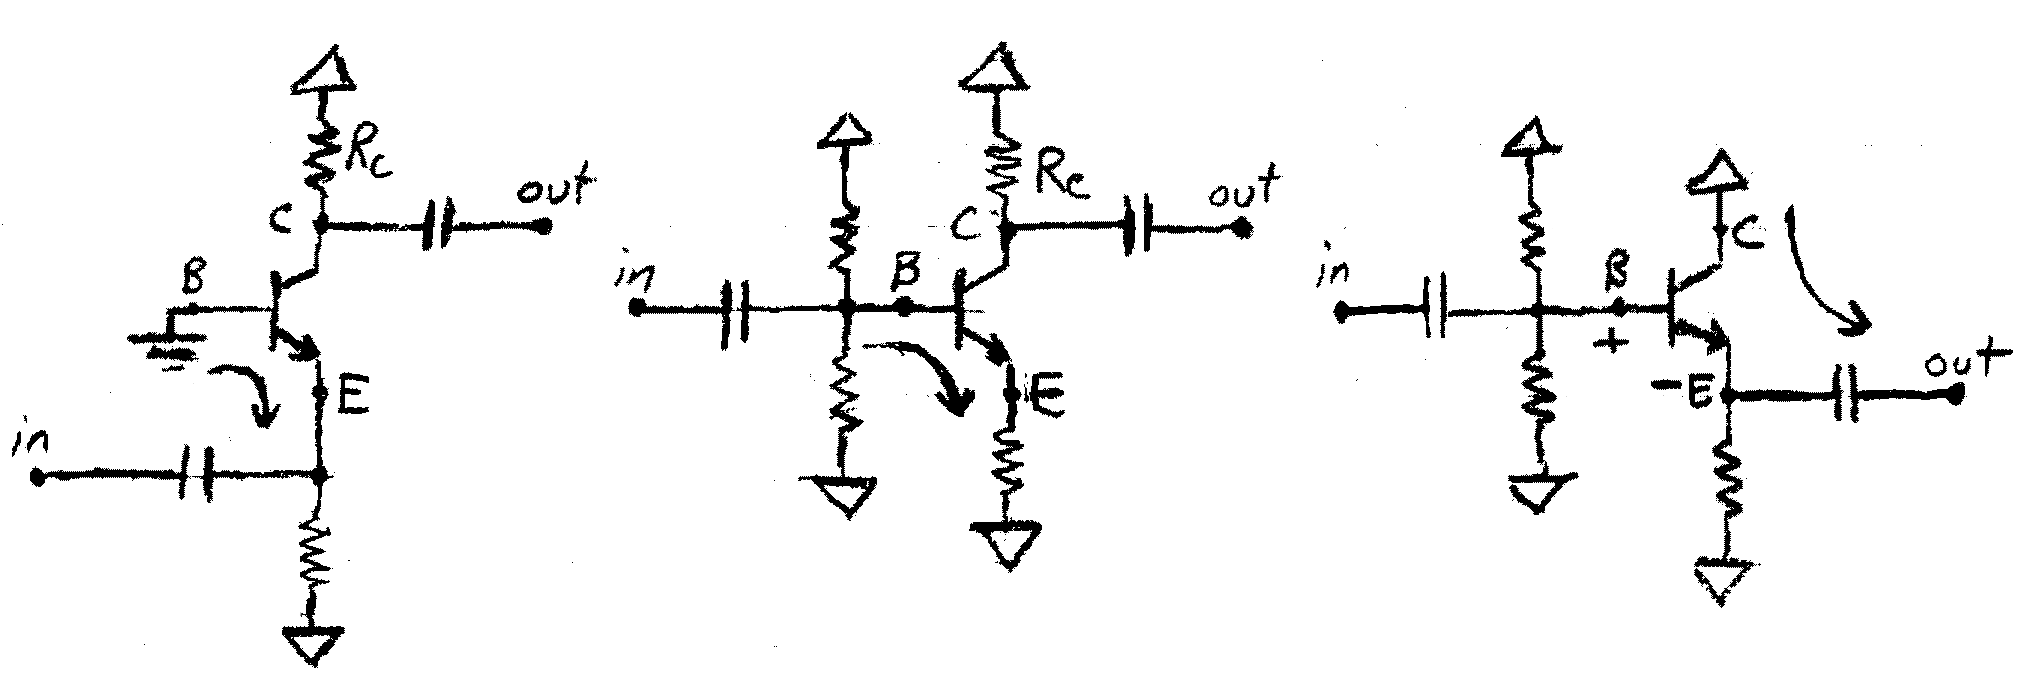
\includegraphics[width=0.75\textwidth]
		{figures/BJTforwardBiasConfigurations.png}
	\caption{
		Common-base (left), common-emitter (middle), and
		common-collector (right) configurations for BJT
		amplifiers.
	}
	\label{BJTforwardBiasConfigurations}
\end{figure}

Each configuration has its tradeoffs. The common-base (CB) configuration is
a good current buffer, with $A_{i}\approx1$ and low input impedance.
The common-emitter (CE) configuration offers the best overall power gain,
but $A_{v}$ and $A_{i}$ may vary with loadings. The common-collector
configuration, or emitter-follower, is a good voltage buffer 
($A_{v}\approx1$) with low output impedance.

The three configurations can be cascaded together to gain the benefits
of each and mask their deficiencies. If cascaded in the order
shown in figure \ref{BJTforwardBiasConfigurations}, from left-to-right,
the resulting 3-stage broadband amplifier would have low input
impedance, good power gain, and minimal output impedance.

A slight modification to the CE and CB configurations in figure
\ref{BJTforwardBiasConfigurations} can apply a filter to the broadband
amplifier; tuning the gain to a narrow frequency set by a tank circuit. 

Because BJTs are minority carrier devices, they act as current amplifiers
without being strongly affected by voltage. For the two configurations
where the output is at the collector (CB and CE), the BJT acts like a
dependent current source feeding the output load and the biasing
resistance $R_{C}$. As a result, the voltage gain for these
configurations is determined primarily by how difficult it is for
the collector current to reach ground; $A_{v}\propto R_{C}||R_{L}$.

The designer can take advantage of the collector current's obstinance
by replacing $R_{C}$ with an impedance that varies with frequency.
Using an inductor and a capacitor in parallel would provide shorts
to ground for DC currents and very high frequency currents. Parallel
LC circuits also have a resonance frequency at which their net 
impedance approaches infinity because power simply oscillates between
the two.
\footnote{For this reason, an $L||C$ circuit is called a tank circuit.}
The result is that the amplifier gain will be very high at resonance,
when impedance is high, but will drop quickly for other frequencies.
\end{document}
